% Author: Emmanuel D. Solis
\documentclass{article}

% Set font encoding for PDFLaTeX, XeLaTeX, or LuaTeX
\usepackage{ifxetex,ifluatex}
\if\ifxetex T\else\ifluatex T\else F\fi\fi T%
  \usepackage{fontspec}
\else
  \usepackage[T1]{fontenc}
  \usepackage[utf8]{inputenc}
  \usepackage{lmodern}
\fi

%--------- Bibliografias --------
\usepackage{apacite} %Trabajar bibliografias APA
\usepackage{natbib} %Agregar Bibliografias

%------------ Estilos -----------
\usepackage{afterpage} %Agregar paginas en blanco
\usepackage{bookmark} %Para bookmark del indice
\usepackage[shortlabels]{enumitem} %Para enumerar con letras
\usepackage{float} %Tablas y posicionamiento de figuras.
\usepackage{fullpage} %Trabajar con menos margenes de pagina
\usepackage{graphicx} %Agregar imagenes
\usepackage{hyperref} %Uso de vinculos
\usepackage{pdfpages} %Incluir pdf externos
\usepackage{xcolor}  %Usar colores

%---------- Herramientas ----------
\usepackage{amsfonts} %Formulas matematicas
\usepackage{amsmath} %Alinear ecuaciones y similar.
\usepackage{listings} %Comandos de Terminal UNIX.
\usepackage{minted} %Incluir codigo de programacion.
\usemintedstyle{one-dark} %Estilo de codigo de programacion.
%\usepackage{sagetex} %Hacer calculos
\usepackage{venndiagram} %Agregar diagramas de Venn

%----------- Idiomas ---------------
\usepackage[spanish]{babel} %Configurar el idioma

\begin{document}

\begin{titlepage}
\centering
{
\includegraphics[width=0.2\textwidth]{logoUCR.png}\par}
\vspace{1cm}
{\bfseries\LARGE Universidad de Costa Rica \par}
\vspace{1cm}
{\scshape\Large Facultad de Ingenier\'ia \par}
{\scshape\Large Escuela de Ciencias de la Computaci\'on e Inform\'atica \par}
\vspace{1cm}
{\scshape\Large CI0128 – Proyecto Integrador: Ingeniería de Software y Bases de Datos \par}
{\scshape\Large Profesoras: Rebeca Obando y Alexandra Martínez \par}
\vspace{1cm}
{\scshape\Huge Reporte: Sprint 3 \par}
\vspace{1cm}
{\Large Nombre del Equipo: Ta' Bueno \par}
\vspace{0.5cm}
{\Large Miembros: \par}
{\Large Emmanuel D. Sol\'is - B97670 (Scrum Master)\par}
{\Large \textit{\color{blue}emmanuel.solispomares@ucr.ac.cr} \par}
{\Large Gabriel Zúñiga - B98755\par}
{\Large \textit{\color{blue}gabriel.zunigaorozco@ucr.ac.cr} \par}
{\Large Jan Murillo - B95447\par}
{\Large \textit{\color{blue}jan.murillo@ucr.ac.cr} \par}
{\Large Kevin Arguedas - B80626\par}
{\Large \textit{\color{blue}kevin.arguedasmuriel@ucr.ac.cr} \par}
{\Large Luis D. Chinchilla - B82227\par}
{\Large \textit{\color{blue}luis.chinchillaotarola@ucr.ac.cr} \par}
\end{titlepage}

\newpage
\tableofcontents

\newpage
%\includepdf[pages={-}]{Enunciado.pdf}

\section{Código Fuente del Sistema}
Se encuentra tanto adjunto en esta carpeta compromida como en el enlace del GitHub
previamente compartido.

\section{Code Review}
A realizarse según nuestra cita para el día viernes 22 de Julio a la 1:30pm.

\section{Unit Testing}
Proyecto de pruebas se encuentra en la carpeta \textit{/Planilla/planilla\_backend\_testing}, 
se adjuntan pruebas para todos los siguientes métodos que fueron todos los métodos públicos
que según el enunciado representaban funcionalidad que había que implementar:

\subsection{Dashboard Controller}
\begin{itemize}
  \item \mintinline{c++}{GetDashboard}
  \item \mintinline{c++}{GetDashboardEmployee}
\end{itemize}

\subsection{Deductions Controller}
\begin{itemize}
  \item \mintinline{c++}{VoluntaryDeductionsBeingUsedByEmployee}
  \item \mintinline{c++}{VoluntaryDeductionsNotBeingUsedByEmployee}
  \item \mintinline{c++}{EstablishVoluntaryDeductionStatus}
  \item \mintinline{c++}{UpdateVoluntaryDeductionEmployee}
\end{itemize}

\subsection{Payment Controller}
\begin{itemize}
  \item \mintinline{c++}{GetEmployeePaymentHistory}
\end{itemize}

\subsection{Projects Controller}
\begin{itemize}
  \item \mintinline{c++}{GetLastPayment}
\end{itemize}

\subsection{Report Controller}
\begin{itemize}
  \item \mintinline{c++}{GetProjects}
  \item \mintinline{c++}{GetReport}
\end{itemize}

\subsection{User Controller}
\begin{itemize}
  \item \mintinline{c++}{GetHours}
  \item \mintinline{c++}{ManageHours}
\end{itemize}

\section{UI Testing}
Videos de prueba de ejecución de las pruebas, junto con el respectivo reporte de los
\textbf{casos de prueba}, ademas del proyecto que crea \textit{Selenium} se encuentran
en la carpeta de este directorio: \textbf{\textit{ui\_testing}}.

Cabe mencionar de forma relevante que se hicieron las pruebas \textbf{grabándolas en el navegador},
no por código, según el enunciado permitía la libertad de ejecutar cualquiera de las dos formas.

\section{Deployment de la aplicación en Azure}
Escogimos la plataforma \textbf{Azure} para el despliegue de la aplicación dado que es la que
mayormente conocemos y donde también teniamos el uso de créditos gratis para poder hacerlo.

Algo importante de estipular es que nuestro repositorio de GitHub originalmente tiene en
el los tres proyectos: archivos de la base de datos, backend y frontend. Por lo que fue
necesario crear dos repositorios copias de estos por aparte, privados, para tener en cada
uno de forma separada el backend y el frontend, y entonces poder hacer el respectivo
\textit{deployment} de cada uno.

Se adjunta en cada seccción los enlaces respectivos para que se pueda ver que el sistema
sí esta accesible.

\subsection{Base de Datos}
Para hacer el \textit{deployment} de la base de datos fue crear una \textbf{nueva base de datos}
en Azure, y usando los scripts que teníamos guardado de la creación de tablas, funciones
y procedimientos, además de los índices y transacciones; pudimos crear la nueva base de datos
sin problema alguno.

\textbf{Enlace del servidor de base de datos:} \href{payroll-database-emmasolis.database.windows.net}{payroll-database-emmasolis.database.windows.net}. Por
favor tengase en cuenta que el servidor de base de datos está en una zona de Azure que por motivos de seguridad
exije que a los usuarios les esté registrada la IP desde la que va a acceder por lo que probablemente
no le permita conectarse pero con gusto puedo reunirme con usted y mostrarle que si está activa.

Tambien se adjunta el \textbf{Connection String}:
\textit{Server=tcp:payroll\-database\-emmasolis.database.windows.net,1433;Initial Catalog=payroll\_database;Persist Security Info=False;User ID=TaBuenoAdmin;Password=UCRecci2022\$;}.

Primero tuvimos que crear un servidor de base de datos, y luego entonces crear la base
de datos para el proyecto. En la Figura \ref{fig:database_server} podemos ver el estado
actual de dicho servidor.

\begin{figure}[h]
 \centering
 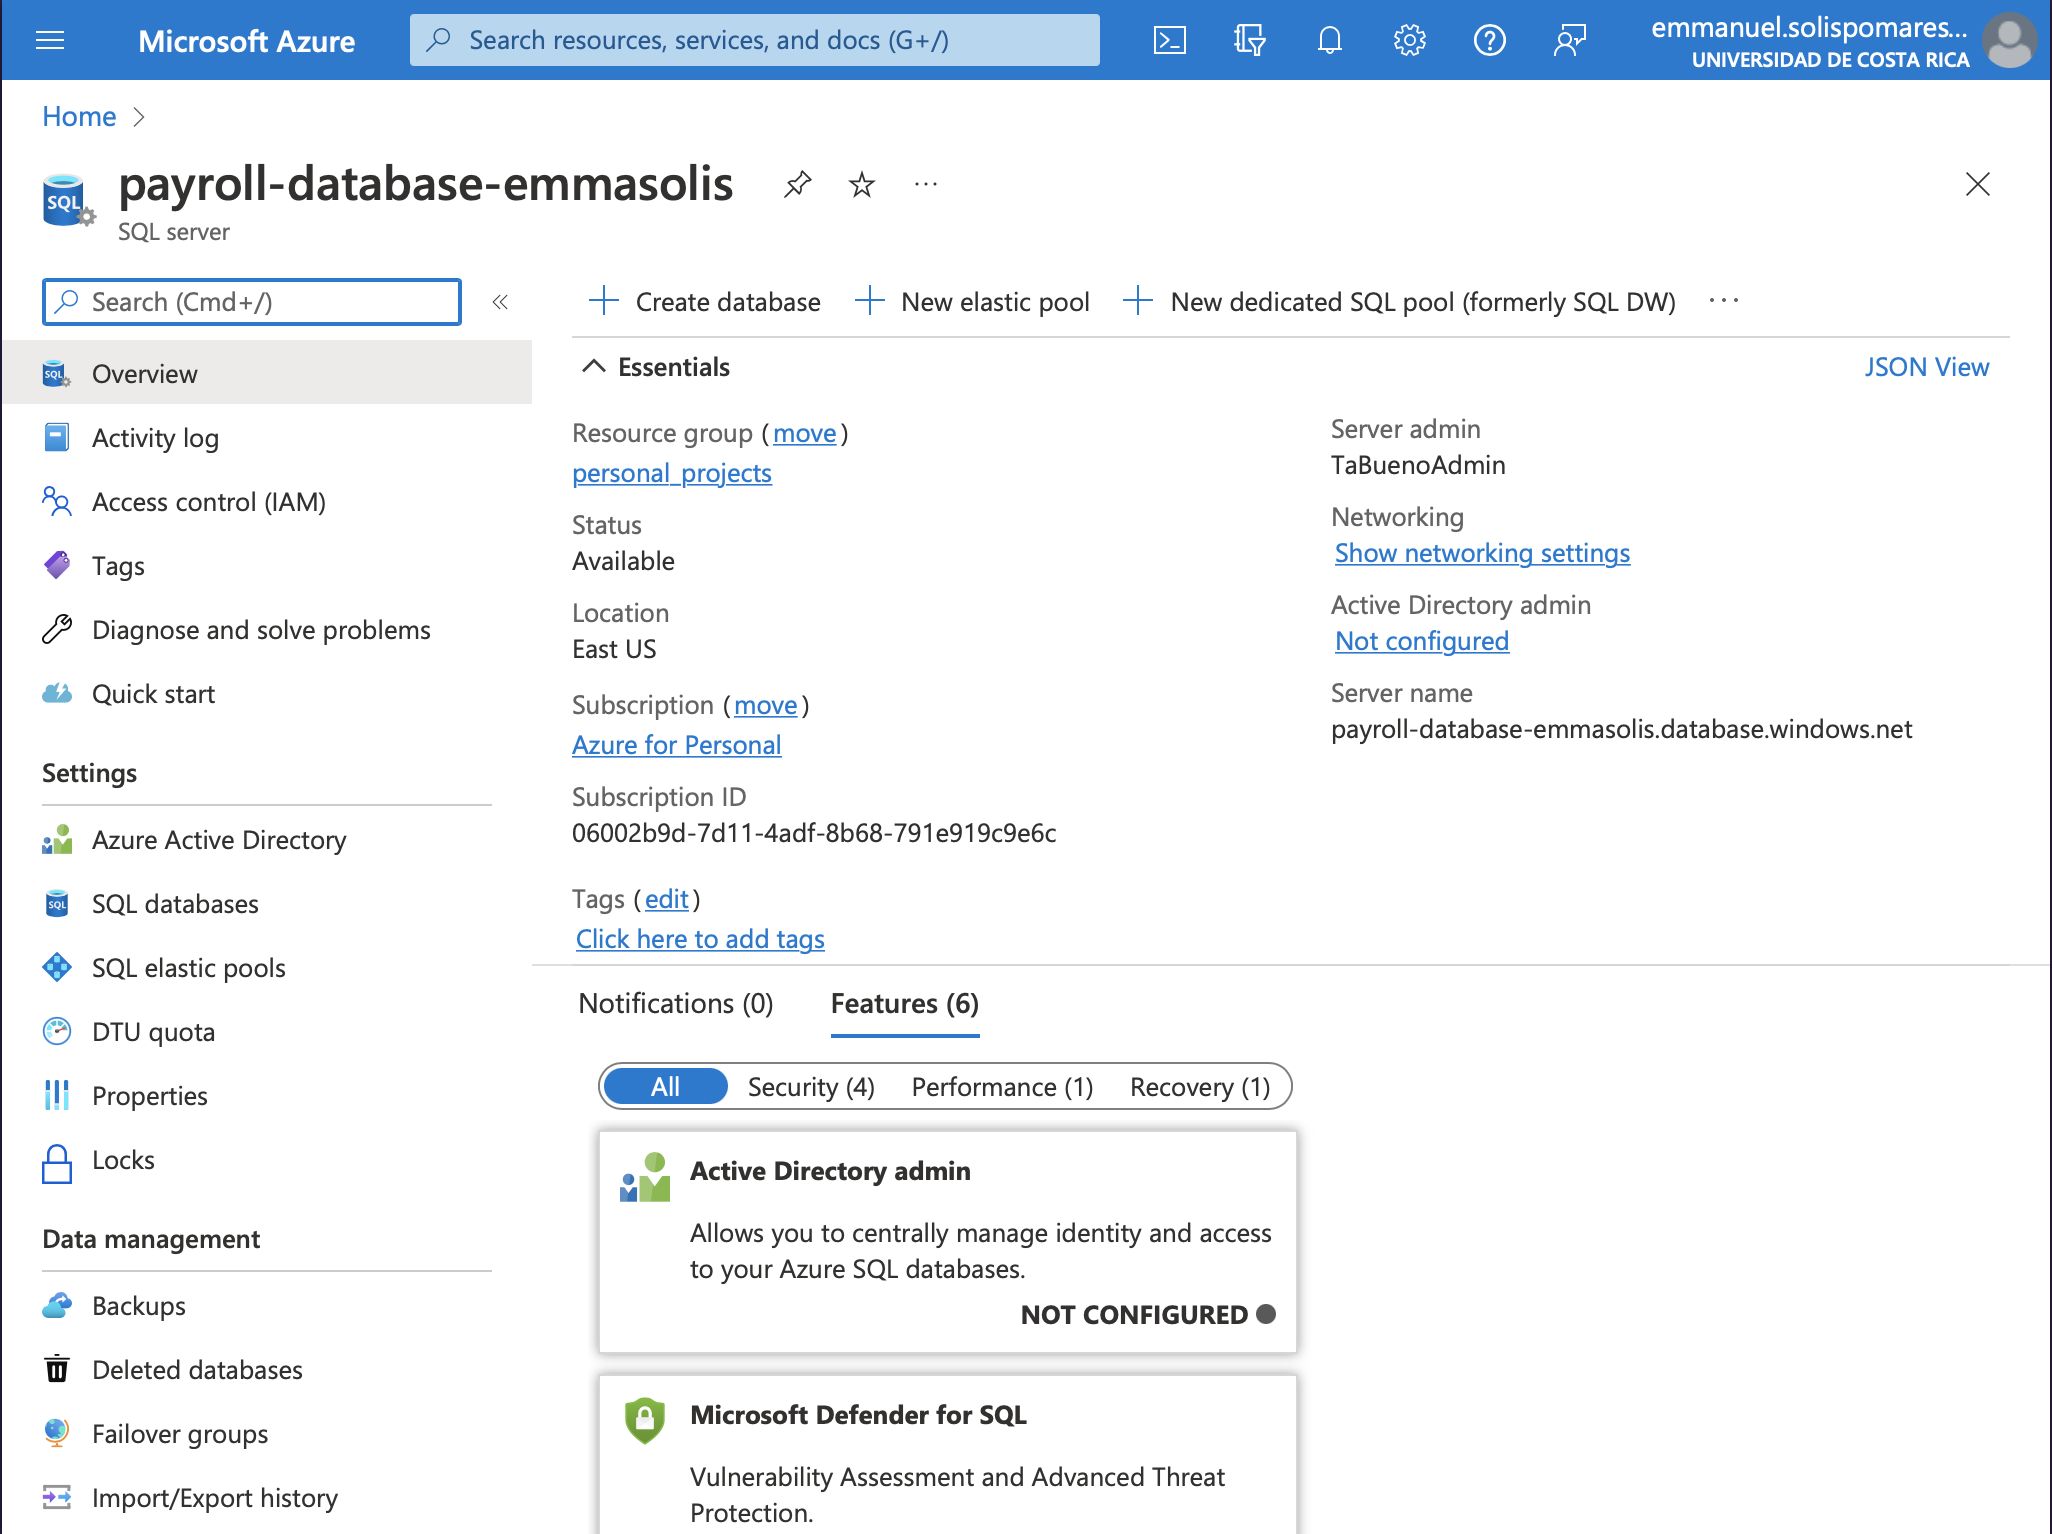
\includegraphics[width=0.95\textwidth]{database_server.png}
 \caption{Vista general del servidor de base de datos en Azure.}
 \label{fig:database_server}
\end{figure}

Una vez que ya teníamos el servidor creamos la base de datos para el proyecto en si,
esta la podemos ver en la Figura \ref{fig:payroll_database}.

\begin{figure}[h]
  \centering
  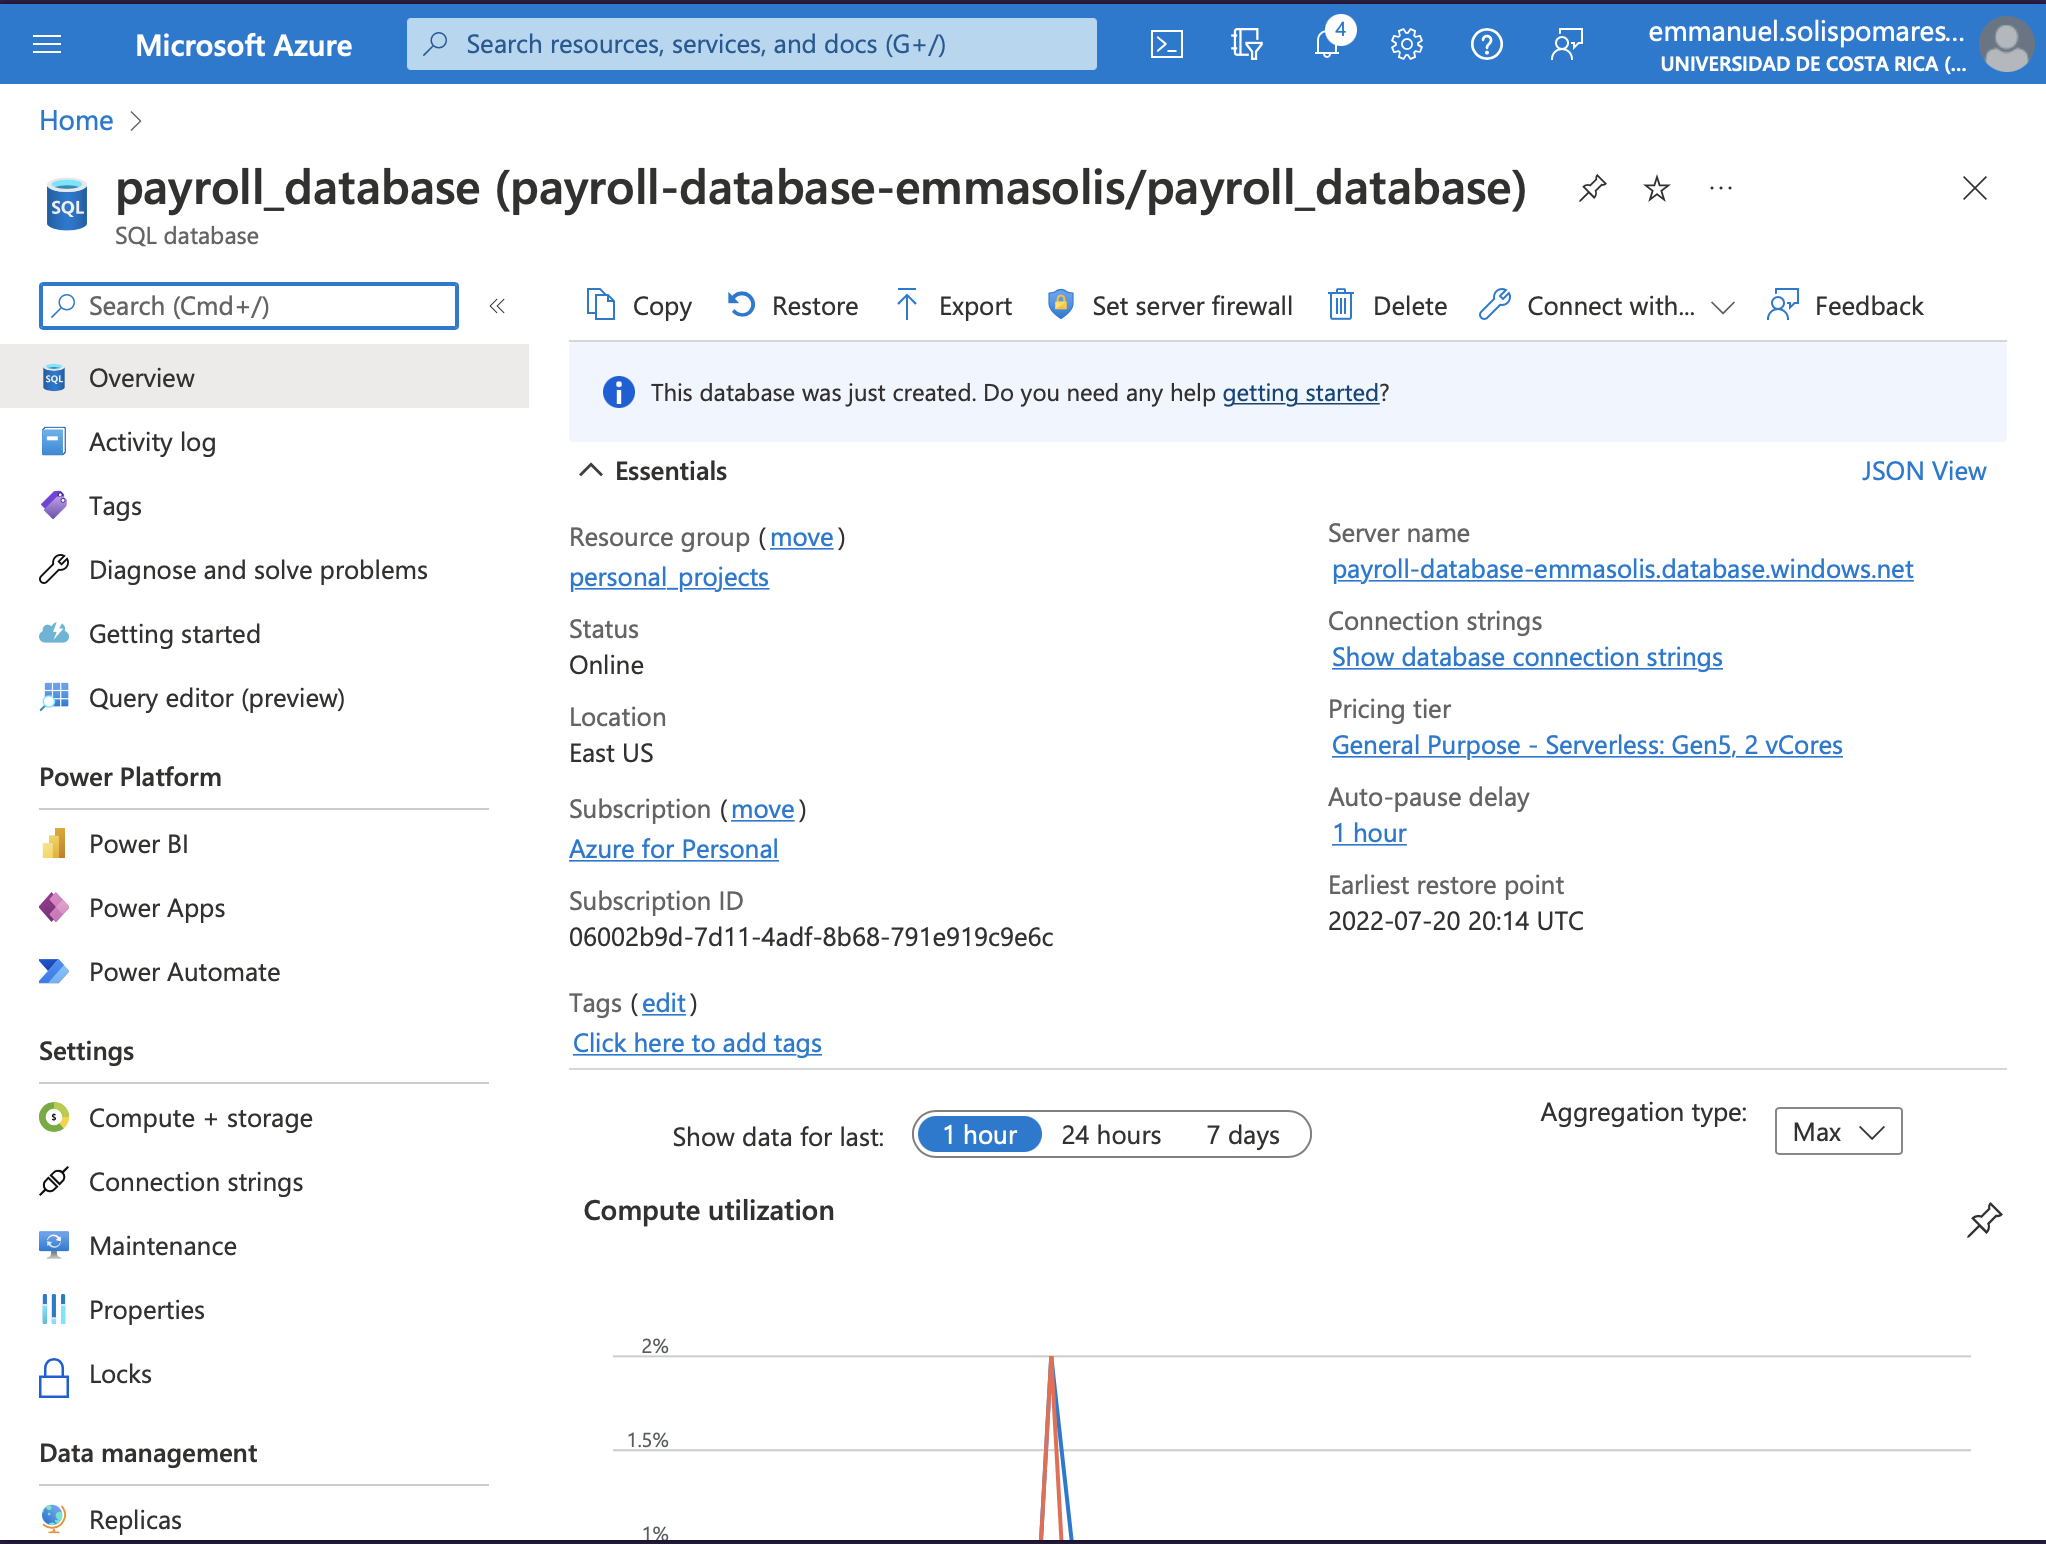
\includegraphics[width=0.95\textwidth]{payroll_database.png}
  \caption{Vista general del de la base de datos \textit{payroll} en Azure.}
  \label{fig:payroll_database}
 \end{figure}

Y al tener estas dos cosas ya teníamos la base de datos en Azure para luego poder ser usada
por las otras dos fases de la aplicación: \textit{Backend} y \textit{Frontend}.

\subsection{Backend}
Para hacer el \textit{deployment} del backend fue más sencillo pues solo fue necesario
tomar el repositorio separado del backend y en Azure crear un nuevo \textit{App Service}
el cuál se le configura que es un .NET API y como esta conectado por medio de GitHub, Azure
la conexión y \textit{deployment} de forma automática por debajo. Con eso ya tenemos
tanto la base de datos como el backend (API) listos y en linea, faltando solo el frontend.

\textbf{Enlace del servidor del Backend:} \href{https://payroll-api-tabueno.azurewebsites.net}{https://payroll-api-tabueno.azurewebsites.net}.

Podemos ver la vista general del backend en la Figura \ref{fig:backend}.
\begin{figure}[h]
  \centering
  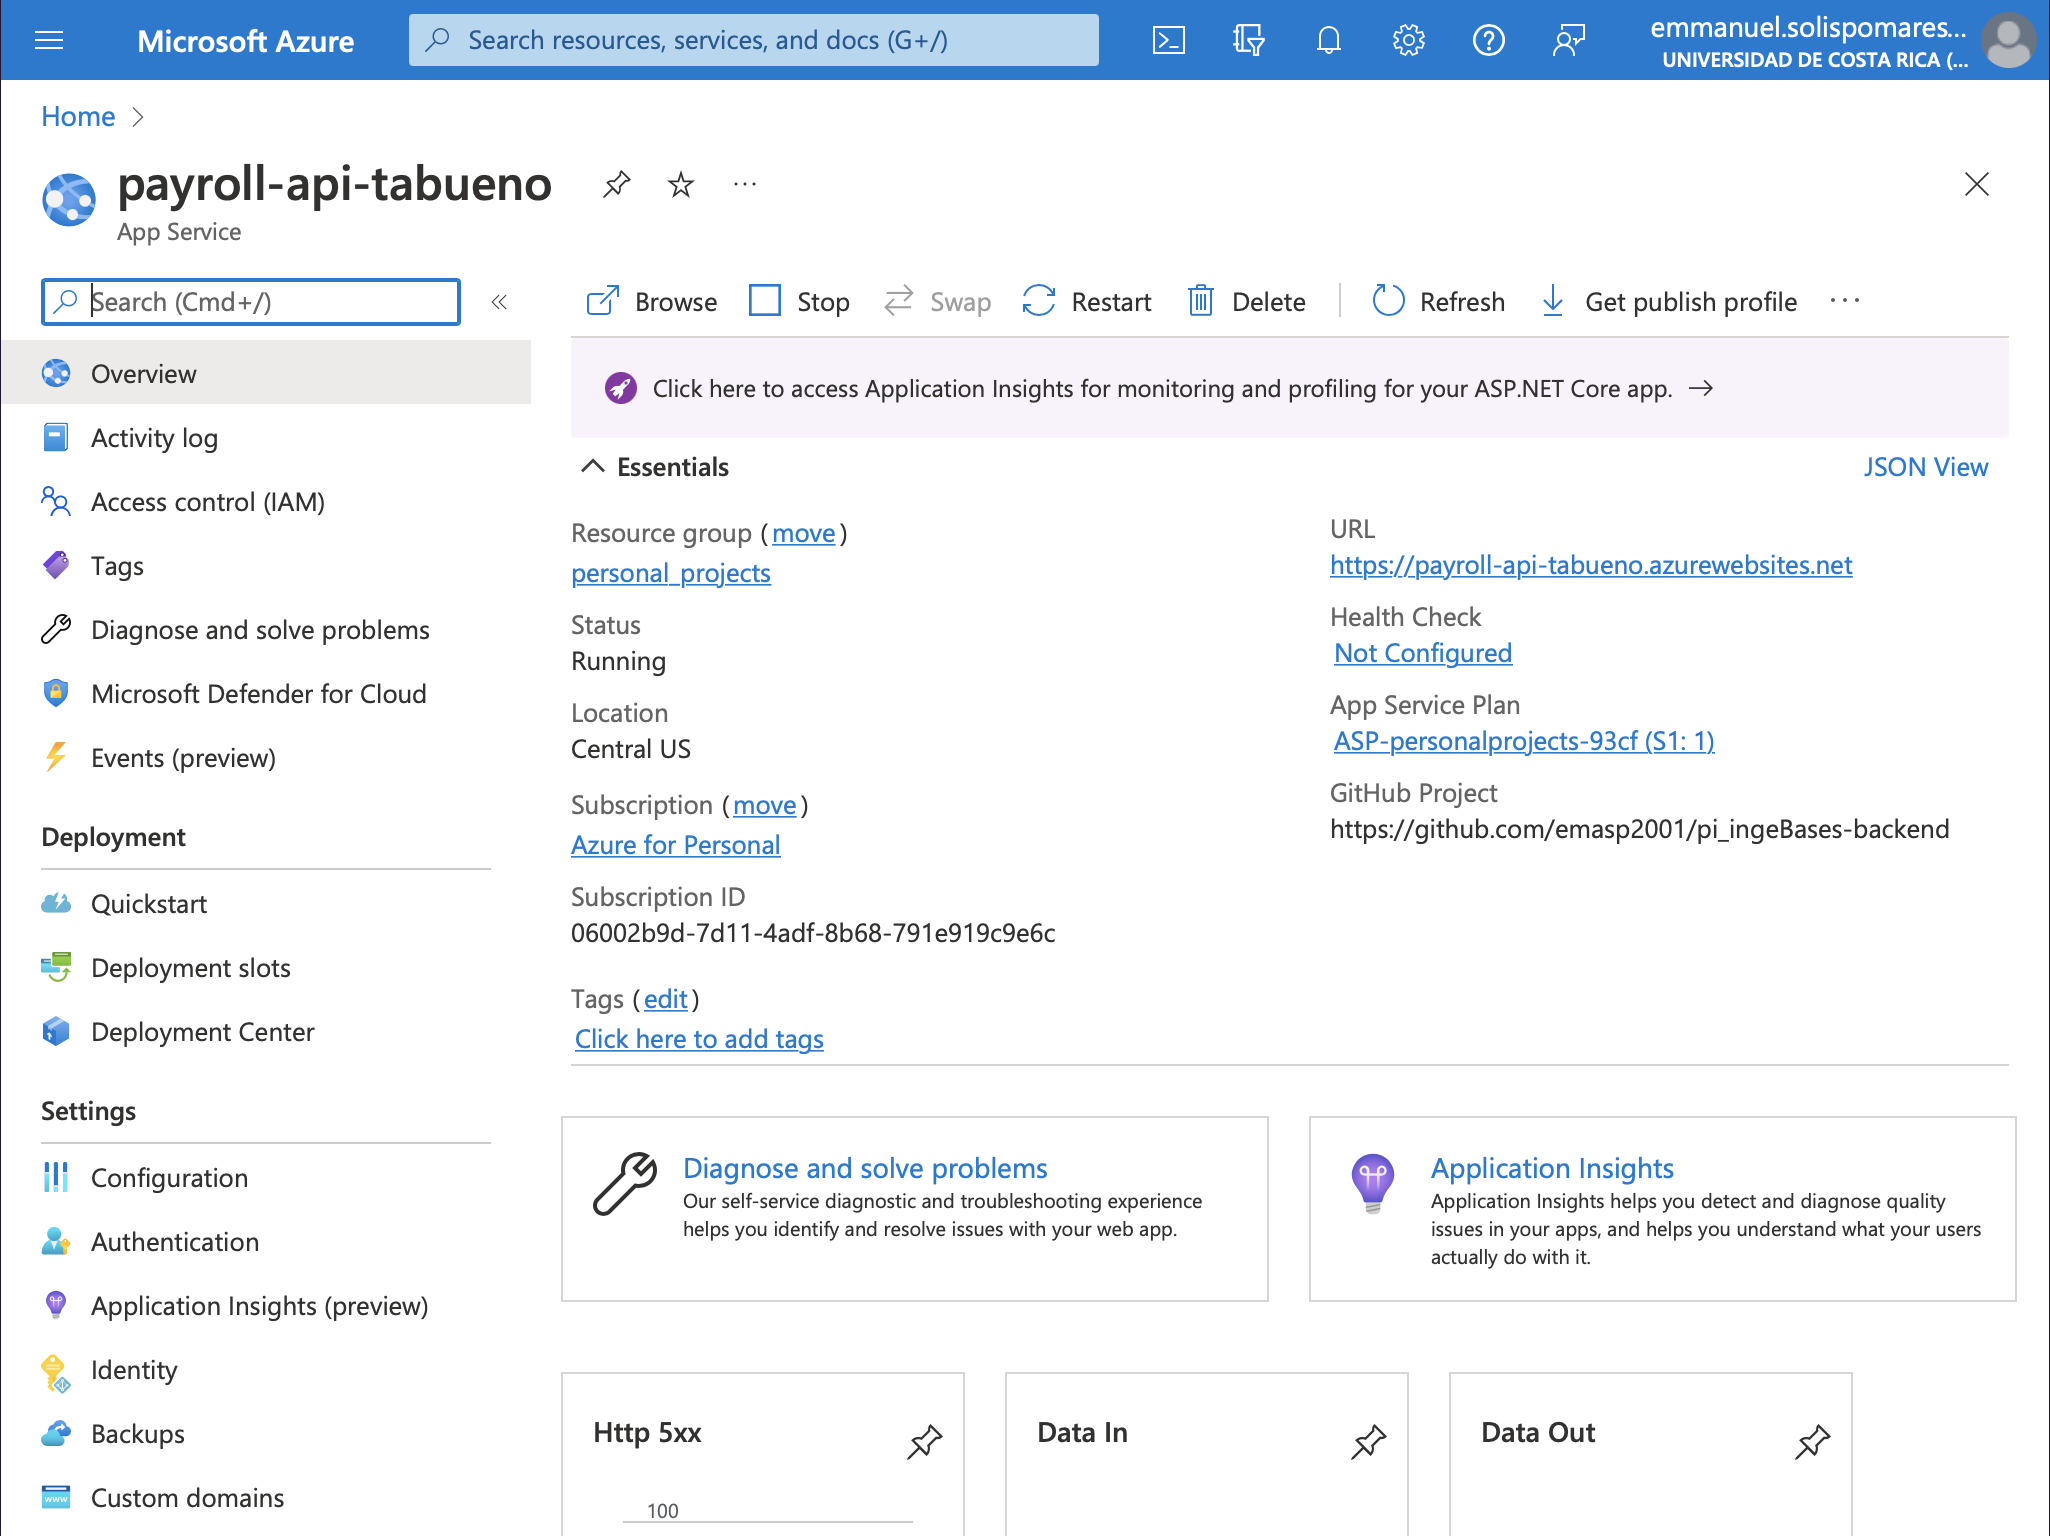
\includegraphics[width=0.95\textwidth]{backend.png}
  \caption{Vista general del Backend API en Azure.}
  \label{fig:backend}
 \end{figure}

 \subsection{Frontend}
En lo que respecta al frontend fue donde tuvimos multiples problemas y fue la unica parte
que no logramos poner en linea del todo, despues de toda una serie de errores llegamos a un
punto donde la aplicaciónn sí se subia correctamente sin embargo el servidor no lograba
identificar cuaál era el puerto que Azure le estaba asiganando a la aplicación, y por lo tanto
tomaba el puerto por defecto que era el 3000 pero esto hacia que no puediera accederse.

\textbf{Enlace del servidor del Frontend:} \href{https://payroll-tabueno.azurewebsites.net}{https://payroll-tabueno.azurewebsites.net}.

Podemos ver en la Figura \ref{fig:frontend} que efectivamente el enlace hacia conexión con
el App Service pero al no encontrar el servidor corriendo en el puerto que debía entonces no devolvía nada.
\begin{figure}[h]
  \centering
  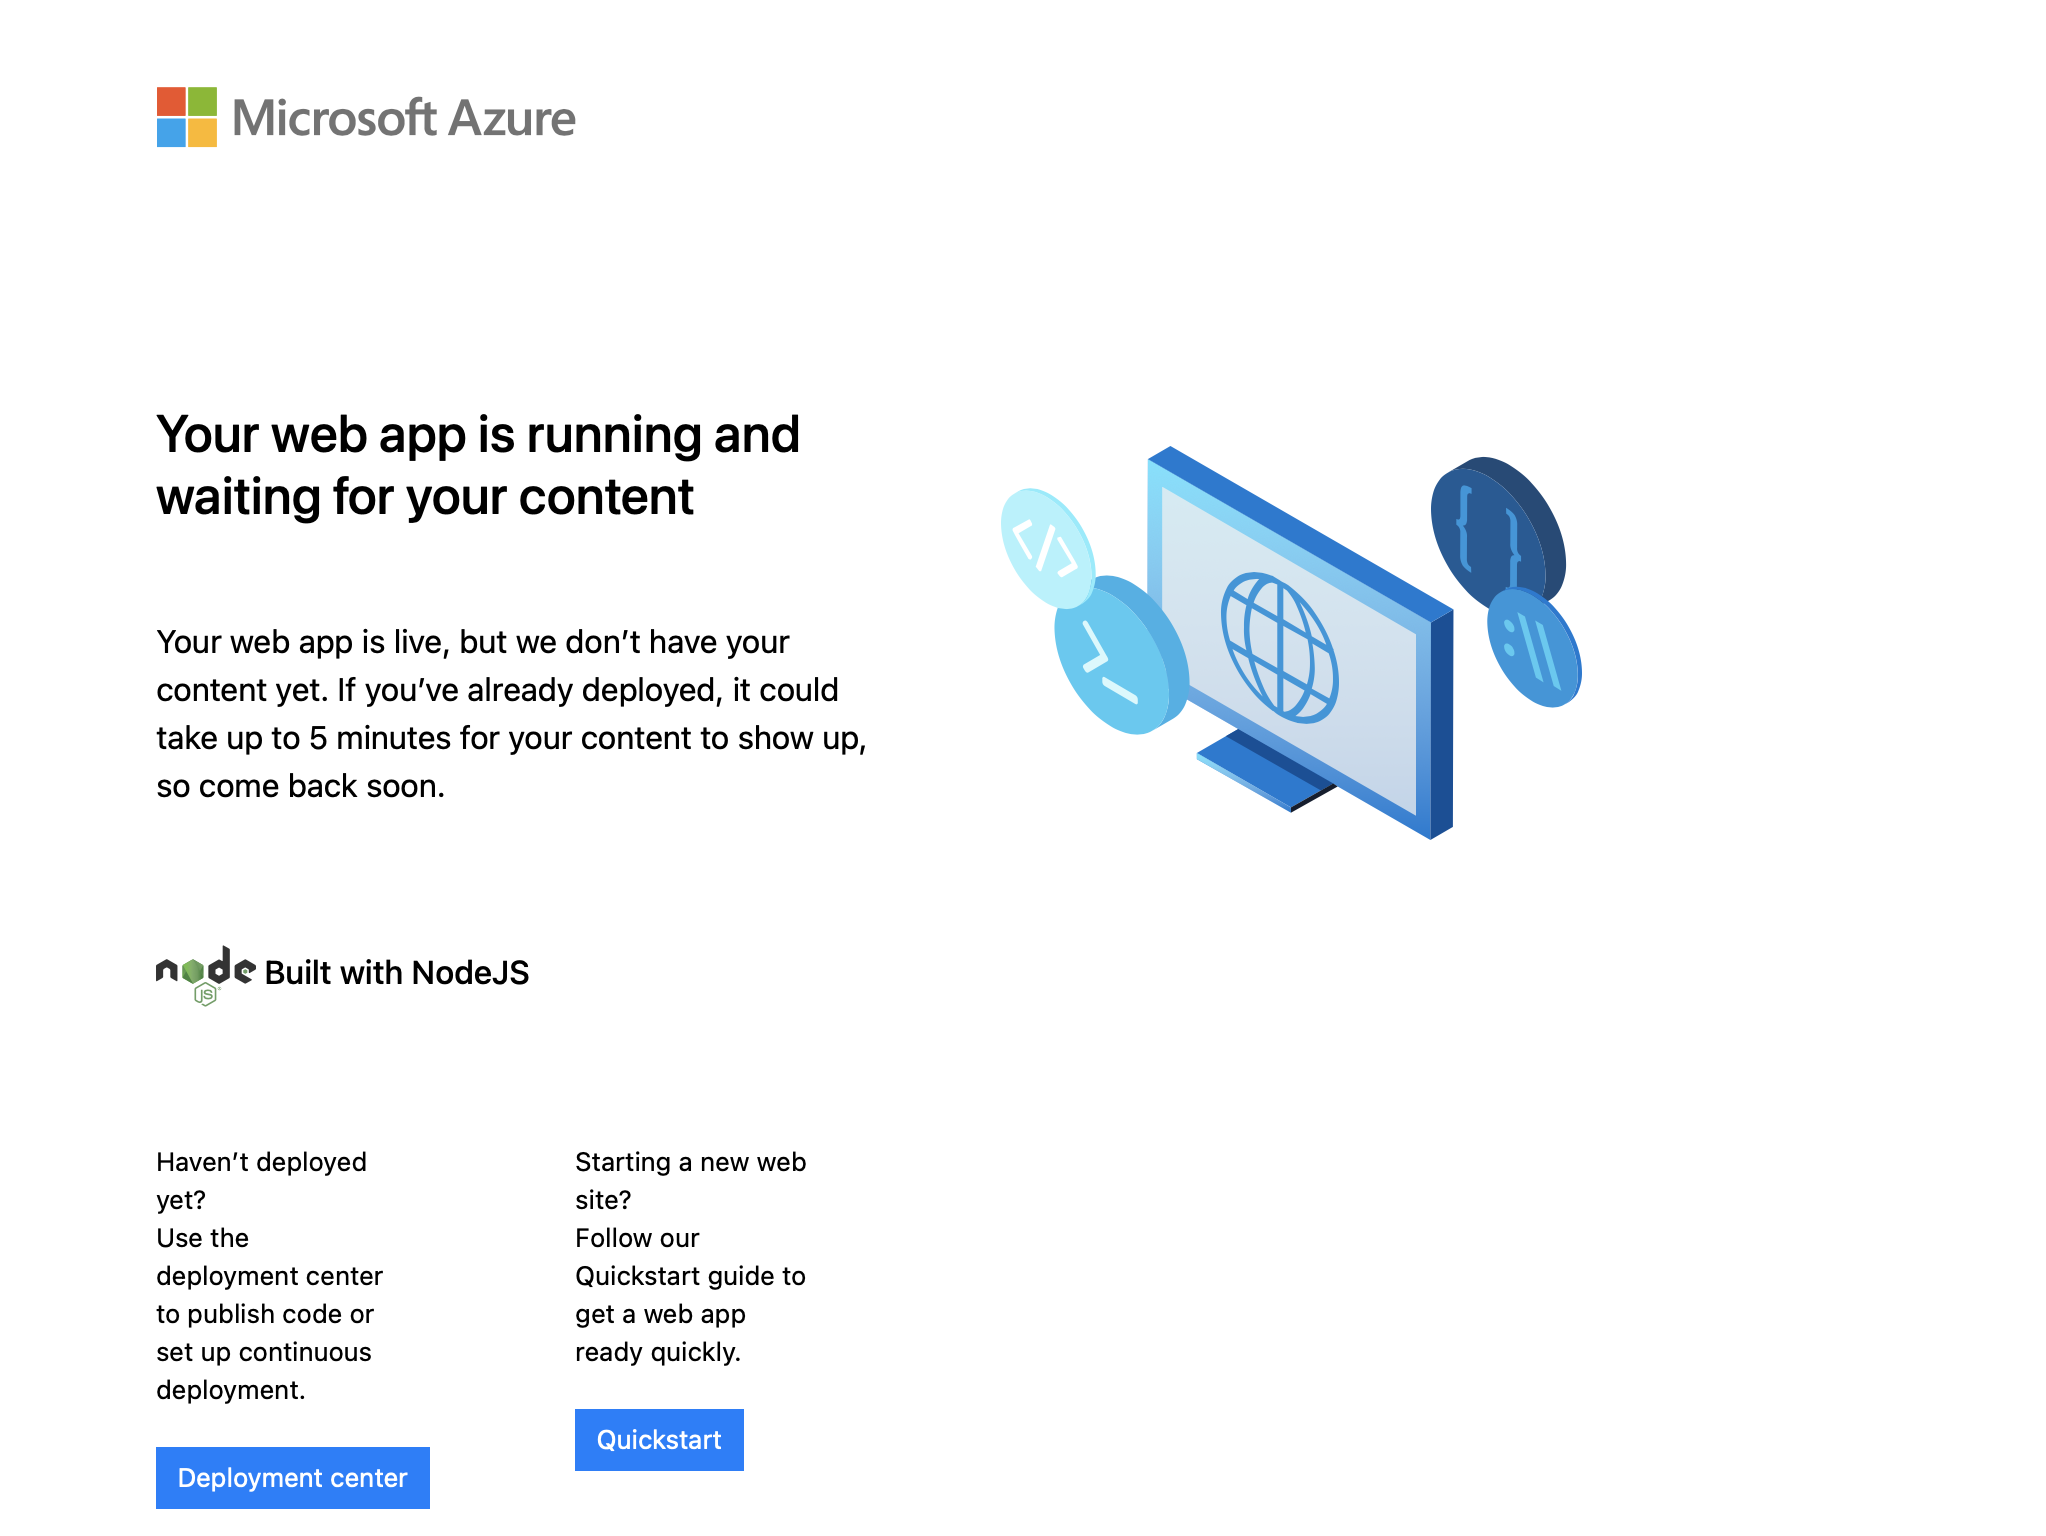
\includegraphics[width=0.95\textwidth]{azure_frontend_status.png}
  \caption{Vista general del Frontend en Azure.}
  \label{fig:frontend}
 \end{figure}

 De forma similar podemos ver en la Figura \ref{fig:git_deploys} que los deployments de la
 aplicación en Azure se estaba haciendo de forma correcta y que incluso pasaba sin errores,
 comprobando así que efectivamente el único problema era que el sistema no estaba escuchando
 en el puerto que debía.
 \begin{figure}[h]
  \centering
  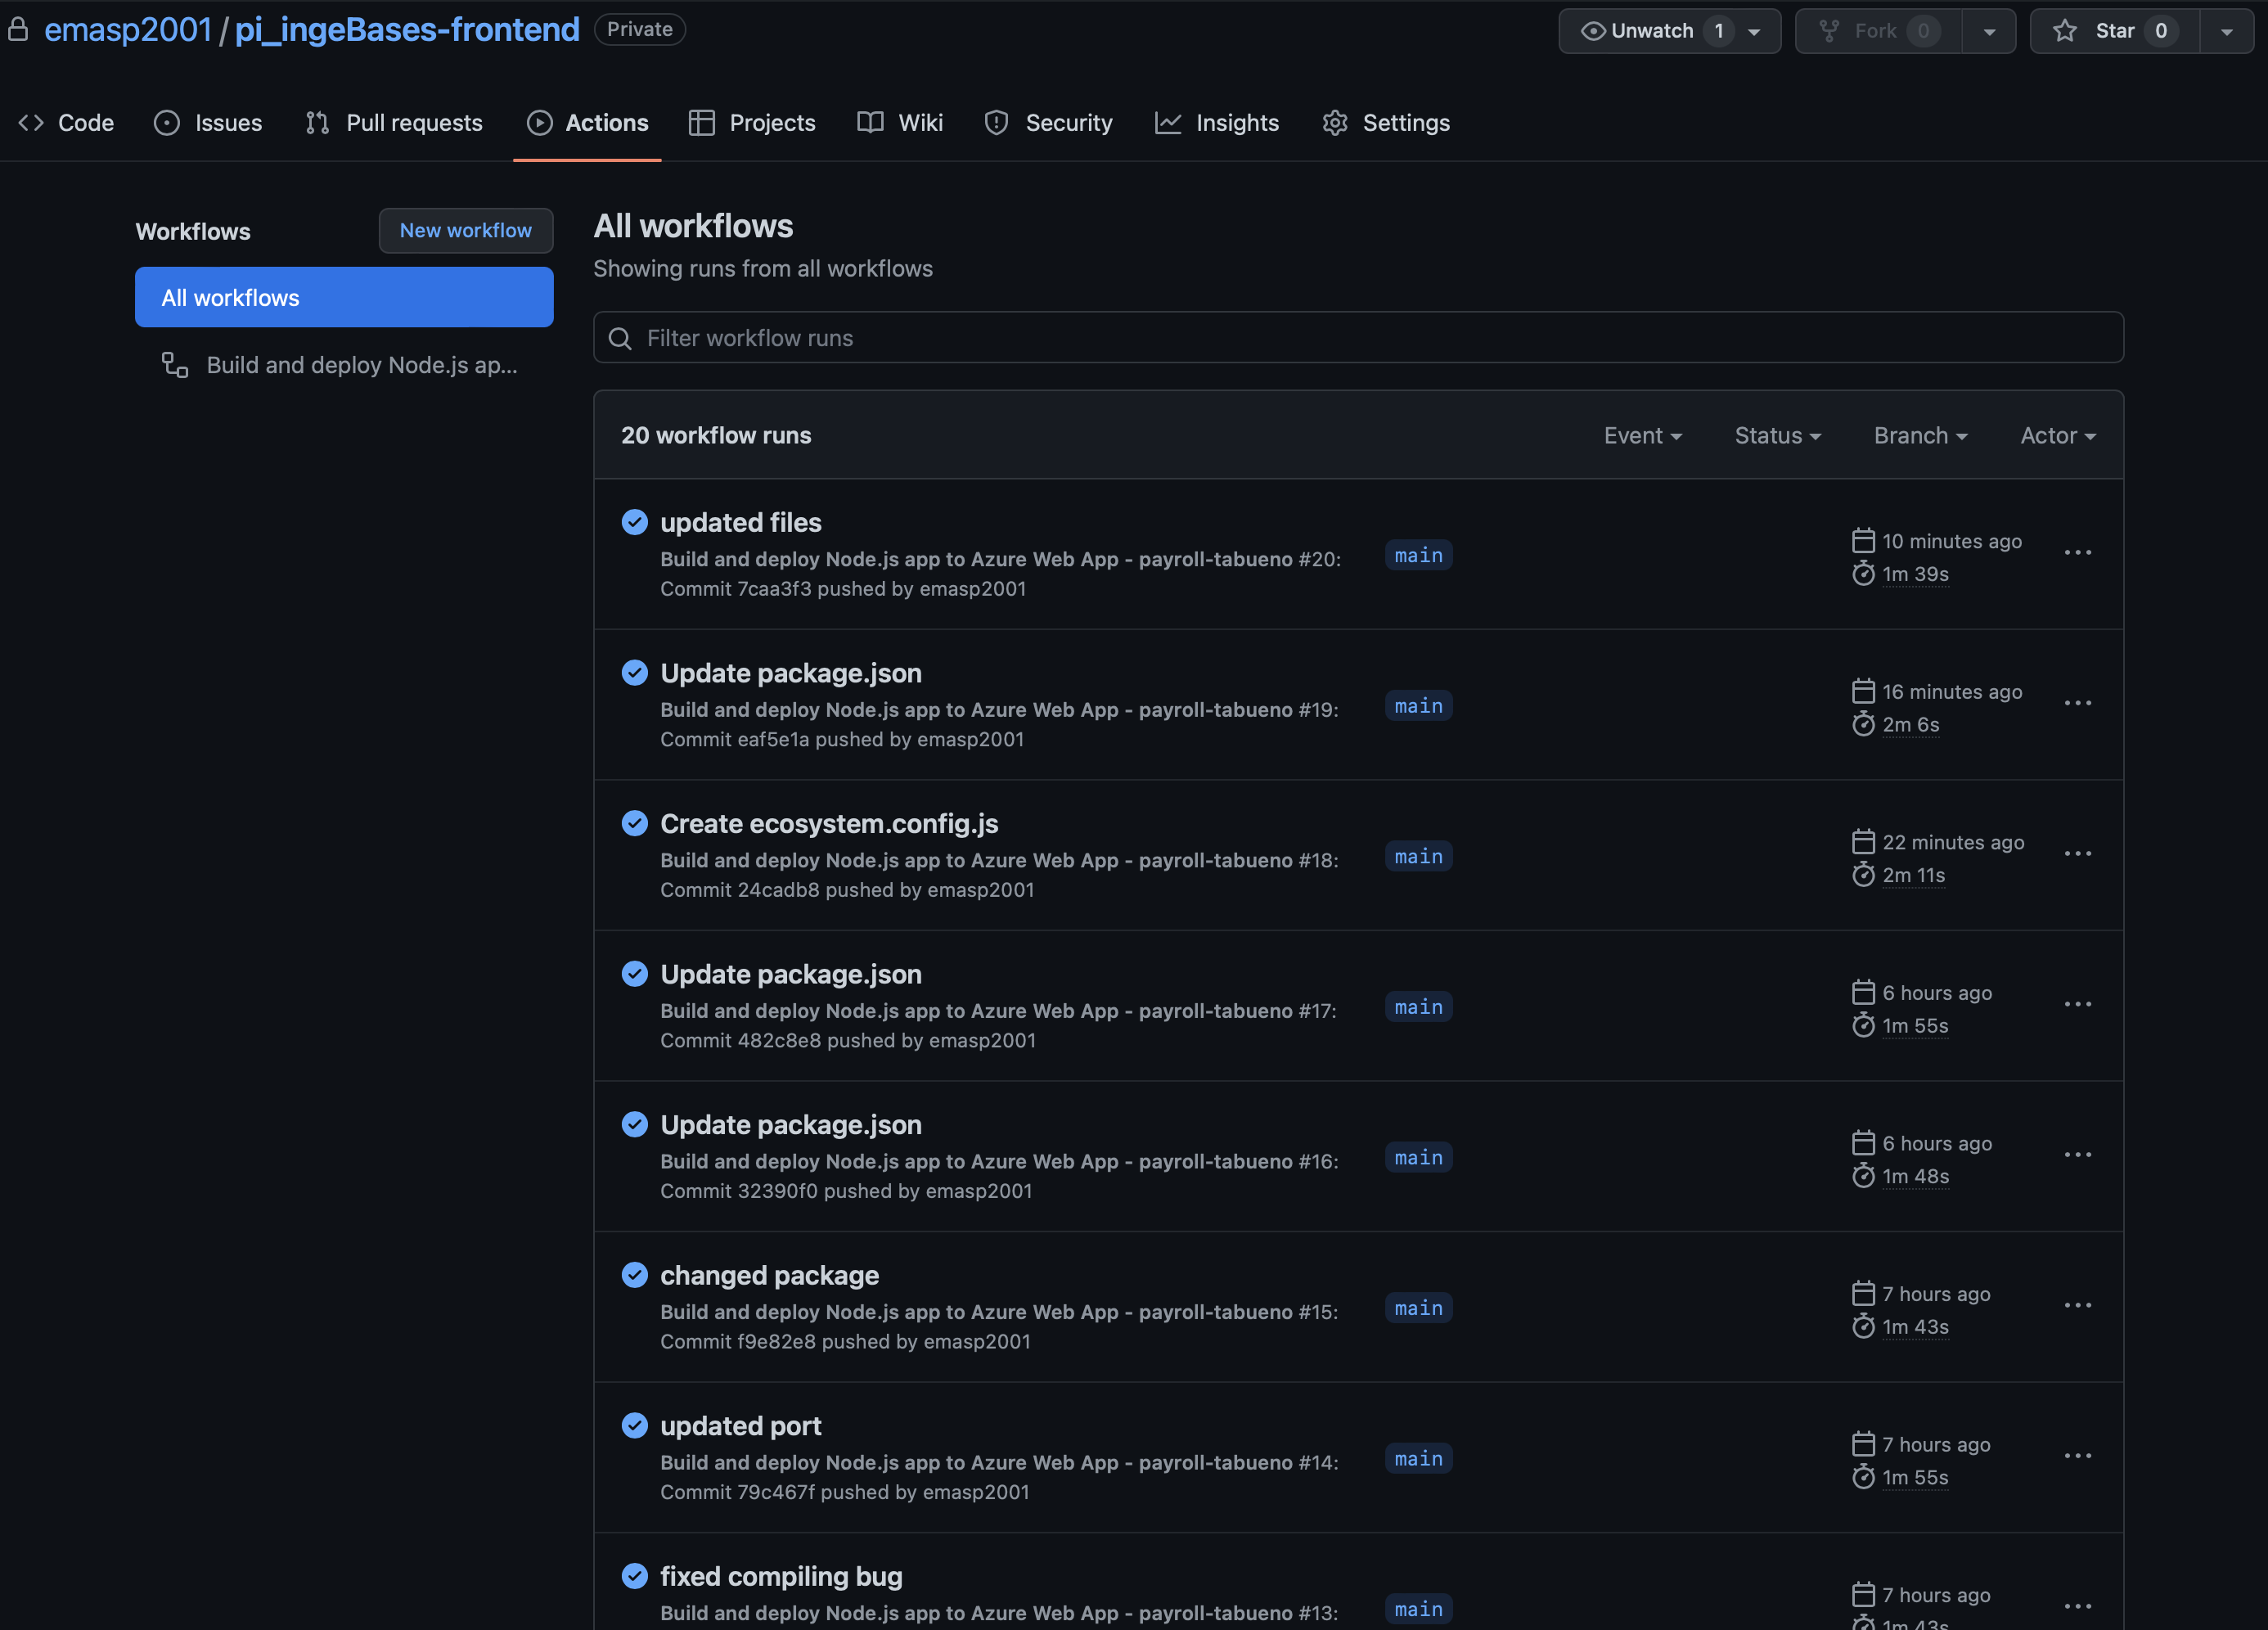
\includegraphics[width=0.80\textwidth]{git_deploys.png}
  \caption{Git Deploys del Frontend.}
  \label{fig:git_deploys}
 \end{figure}

 \subsubsection{Problemas encontrados al subir el Frontend}
 \begin{itemize}
  \item Habían \textbf{archivos que evitaban que el servidor compilaba} porque el nombre de una
  carpeta de donde se traían componentes estaba con el \textbf{mismo nombre pero una letra en mayúscula en vez de minúscula},
  este error no había sido detectado antes porque se corría en Windows y el Windows como no distingue
  entre mayúsculas y minúsculas, entonces no se detectaba el error. Este errror nos consumió 
  bastante tiempo para poder ser encontrado.

  \item El \textbf{script del deployment no funcionaba} correctamente, tenía ciertas operaciones
  que hacía cada deployment increiblemente largo, aproximadamente 2 horas, por lo que hasta el más
  pequeño cambio en el frontend hacia que tuvieramos que esperar 2 horas extras.

  \item Se intentó hacer la \textbf{IP de la casa de Emmanuel como publica} como un método
  alternativo para hacer el sistema accesable a todo el internet, sin embargo este redireccionamiento
  no dió resultado, principalmente porque las IP públicas tienden a cambiar mucho y muy seguido, y
  porque los certificados SSL para conexiones HTTPS se mostraban como inseguros.

  \item El compañero \textbf{gabriel también intentó hacer una IP pública} para el frontend, pero no 
  se pudo dado que salía el certificado SSL como invalido.

  \item Al final se logró subir la aplicación a Azure pero el \textbf{servidor no detectaba cuál era el puerto que debía tomar}
  por lo que por defecto tomaba el 3000, pero ese no era el que estaba escuchando el enlace de
  Azure por lo que aunque el servicio estaba en linea y sin errores no se lograba acceder a esta misma.
 \end{itemize}

\section{Sprint Backlog}
Se encuentra en el siguiente enlace de la profesora Rebeca Obando: \url{https://ingesoftg001.atlassian.net/jira/software/projects/TB/boards/5/backlog}.
Con todos los requerimientos solicitados según el enunciado.

\section{Entregable de las ceremonias}
Se encuentra adjunto en el archivo de esta carpeta llamado \textbf{ceremonias\_scrum.pdf}. Ademas se
adjunta el video respectivo de la reunión \textit{Sprint Retrospective} con el nombre
\textbf{retrospective\_meeting.mp4}.
También tenemos el gráfico \textbf{Sprint burndown chart} en la Figura \ref{fig:burndown}.
\begin{figure}[h]
  \centering
  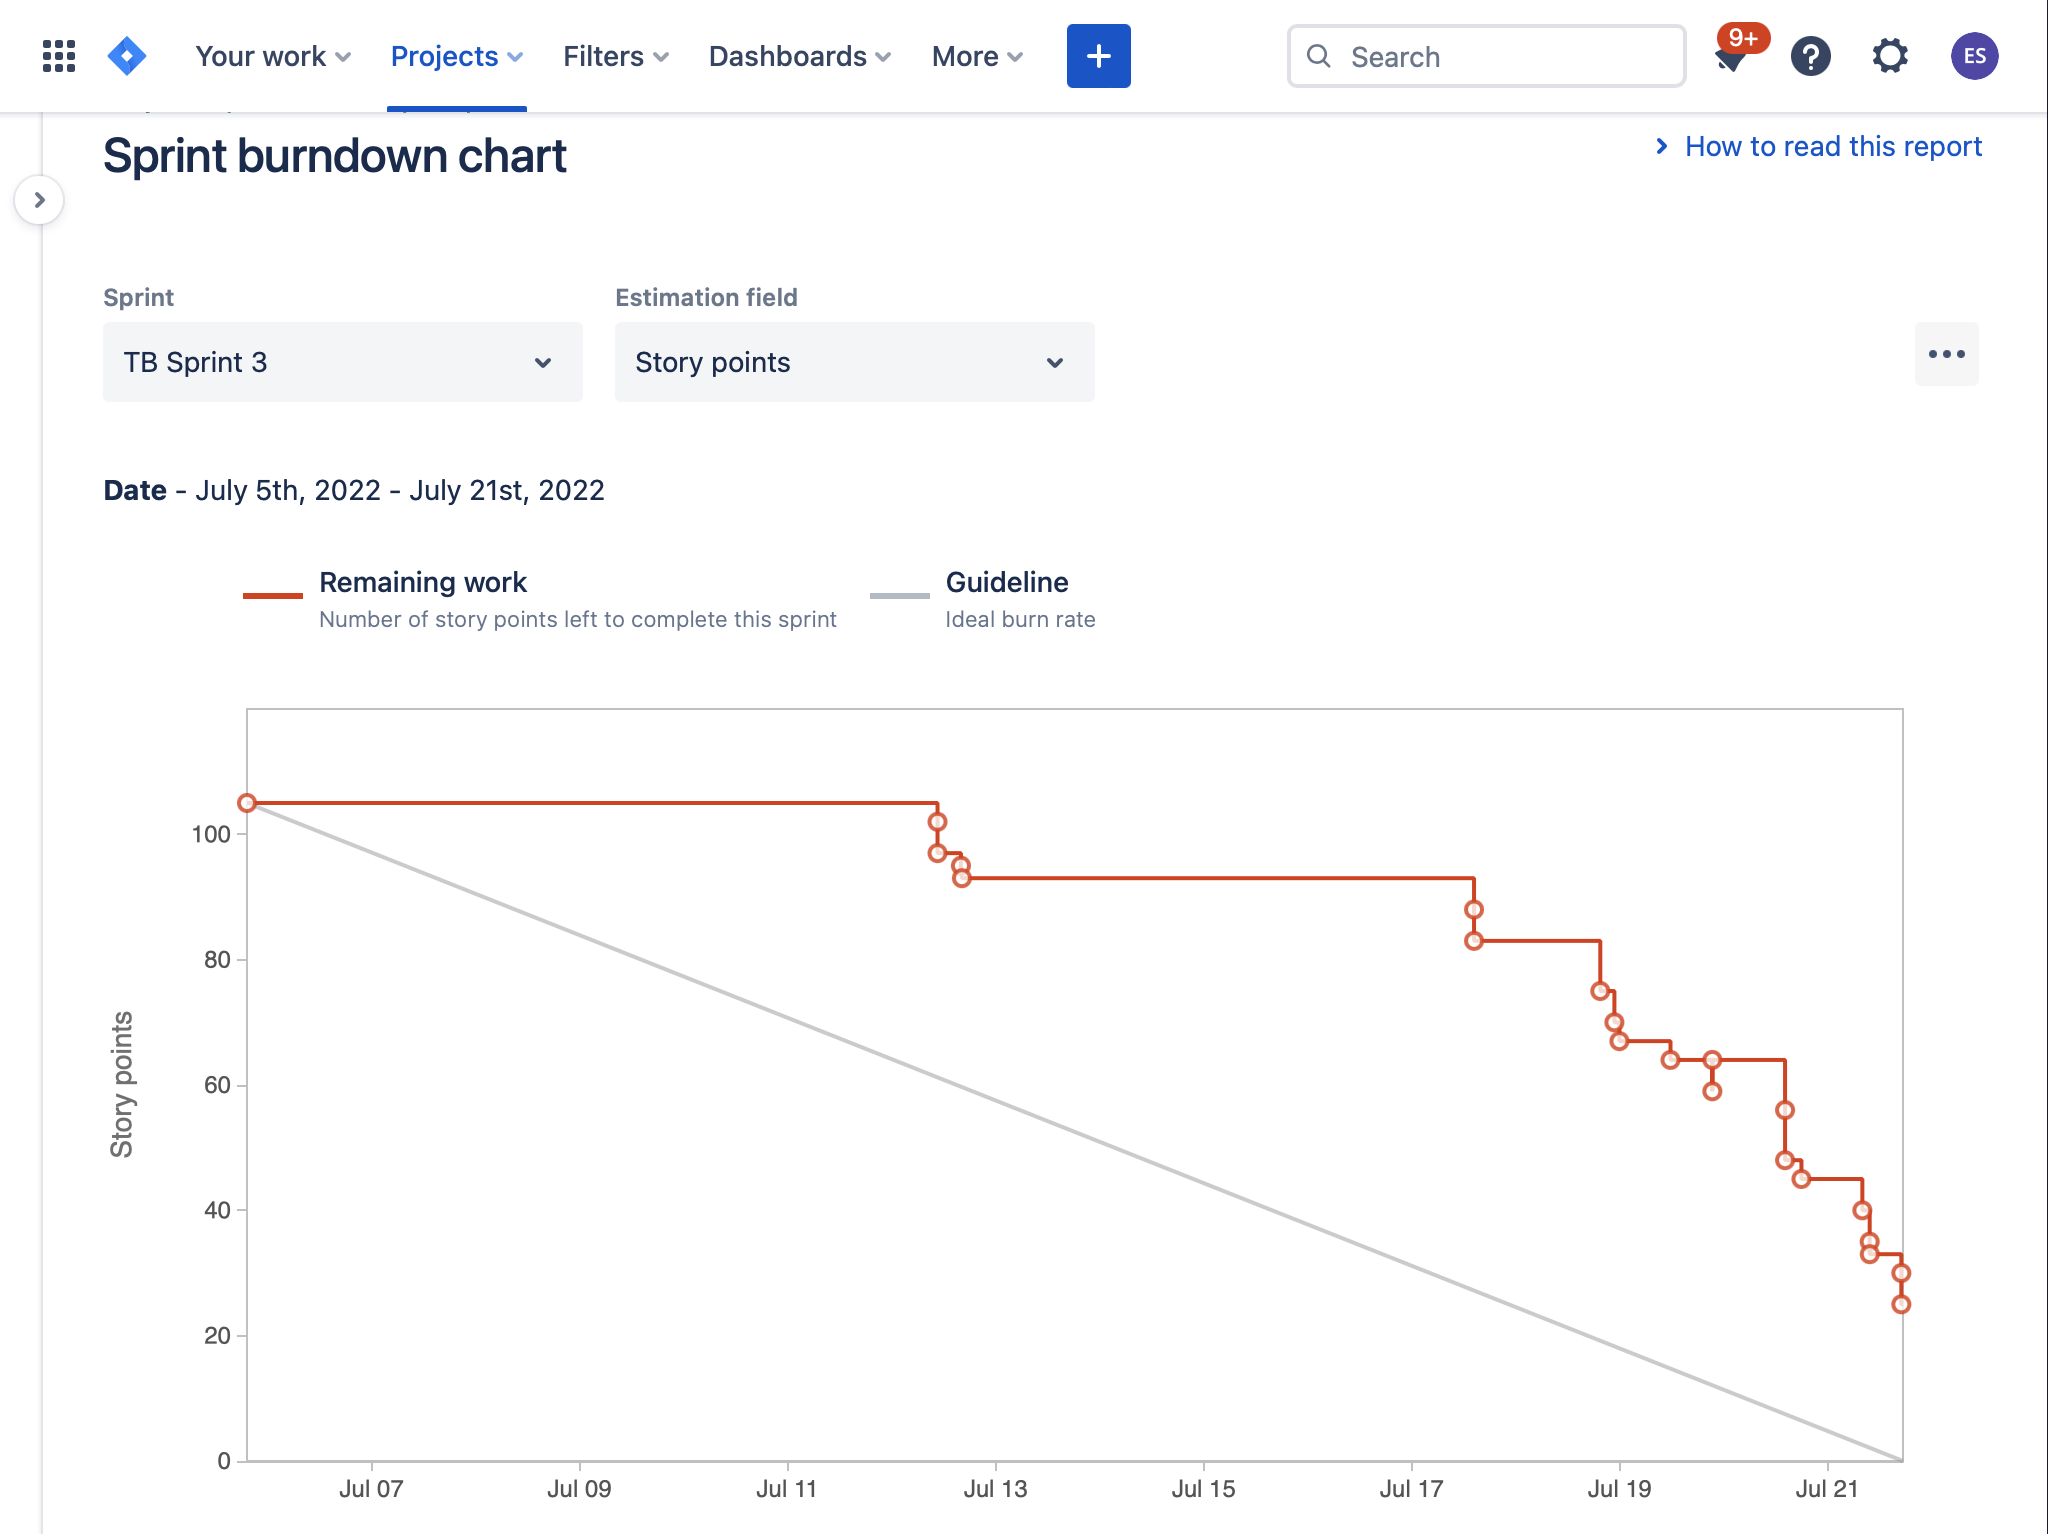
\includegraphics[width=0.80\textwidth]{burndown.png}
  \caption{Gráfico de Burndown del Sprint 3.}
  \label{fig:burndown}
 \end{figure}

\section{Mock Ups}
Se encuentran en el archivo \textit{mock\_ups.pdf}. Para este sprint 3 correspondían 
los \textit{Mock Ups} de los reportes y los dashboard tanto del empleado como del empleador.

 \section{Implementación de la Base de Datos}
Nuestra base de datos \textit{Ta Bueno} se encuentra implementada con las tablas que teníamos
en los diagramas de Modelo Entidad\-Relación y Lógico que fueron previamente presentados y aprobados por la profesora 
Alexandra.

Se agregaron las respectivas funcionalidades de los índices y transacciones, y todo lo necesario
según esta entrega; cabe mencionar que la base de datos ha sido ampliamente presentada para revisión
a la profesora, y la profesora ha aprobado el diseño e implementación que hemos tenido.

Se adjuntan a demás todos los \textit{scripts} de todo los creado en la base de datos,
este se encuentra en la carpeta \textbf{database\_scripts}. Cabe mencionar que la base de datos
que se enceuntra en Azure es una replica exacta de esta base de datos por lo que con revisar
esta que se encuentra en los servidores de la \textit{Escuela de Ciencias de la Computación e Informática}
es suficiente.

\section{Presentación durante Sprint Review}
Se realizará la exposición el día 27 de Julio del 2022 debido a problemas técnicos con la 
base de datos fuera de nuestro alcance.

\section{Autoevaluación y Coevaluación}
Cada miembro del equipo se encarga individualmente de enviar su documento de auto y coevaluación.

%\begin{figure}[h]
%  \centering
%  \includegraphics[width=0.65\textwidth]{SystemCalls.png}
%  \caption{Funcionamiento interno de una interrupción al Sistema Operativo \cite[]{whatSysCalls}.}
%  \label{fig:HowWorksSysCalls}
%\end{figure}

%---------------------- Document Ending ----------------------------------
\newpage
\bibliographystyle{apacite}
\bibliography{bibliography.bib}
\end{document}